\section[Spektrometrie neutronů]{Spektrometrie neutronů pomocí Bonnerových sfér a scintilačních detektorů na bázi odražených jader}

\subsection{Bonnerovy sféry}

Spektrometrie neutronů metodou Bonnerových sfér funguje na principu měření odezev neutronového zdroje při různých moderujících prostředích. Scintilační detektor LiI je citlivý na tepelné neutrony, proto se provedou různá měření s různými moderujícími prostředími, v tomto příkladě se kolem detektoru umisťují PE sféry o různých poloměrech. Tyto sféry vytváří z rychlých neutronů neutrony tepelné, které je detektor schopen zaznamenat, přičemž platí, že s rostoucí tloušťkou sféry nejprve roste moderující vlastnost, a tím i roste odezva v detektoru, nicméně po překročení určitého poloměru začne převažovat absorpce neutronů v PE (stínicí schopnost) a odezva opět klesá.

Další roli hraje i moderace pomocí odrazu v místnosti. Proto se pro každou sféru provádějí 2 různá měření:

\begin{itemize}
    \item První probíhá pouze umístěním neutronového zdroje do určité vzdálenosti od detektoru.
    \item Při druhém měření se mezi detektor a neutronový zdroj vloží stínicí přepážka, která zabrání přímému vstupu neutronů ze zdroje do detektoru (detektor tak zaznamenává pouze neutrony odražené v místnosti).  
\end{itemize}

Vzájemným rozdílem těchto četností je poté možné určit odezvu, kterou poskytuje přímý svazek neutronů z neutronového zdroje.

Bonnerovy sféry jsou tvořeny:

\begin{itemize}
    \item Kulovými obaly z moderátoru různého průměru (typicky 5--30 cm).
    \item Centrálním detektorem umístěným ve středu každé sféry.
\end{itemize}

Každá sféra má odlišnou energetickou odezvu, což umožňuje rekonstruovat neutronové spektrum.

\begin{figure}
    \centering
    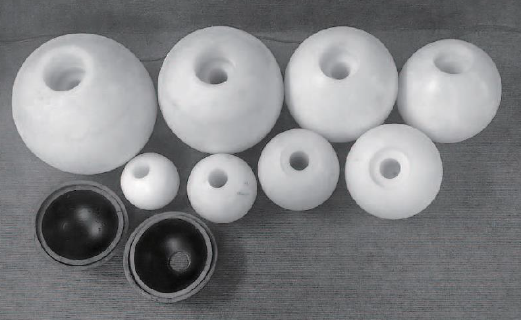
\includegraphics[width=0.75\linewidth]{img/BonorovySféry.png}
    \caption{Bonnerovy sféry}
    \label{fig:enter-label}
\end{figure}

\subsection*{Unfolding energetického spektra}

Po získání odezev pro různé poloměry sfér následuje proces zpětné dekonvoluce, známý jako \textit{unfolding}, který slouží k určení energetického spektra neutronů. K tomu se využívají specializované programy, například \textbf{SAND}, a vhodné aplikační knihovny.

Unfolding je však složitý proces:

\begin{itemize}
    \item Jedná se o nepodmíněnou úlohu s teoreticky nekonečným počtem řešení.
    \item Aby bylo možné stanovit pravděpodobné spektrum, využívá se tzv. \textit{a priori spektrum}, což je odhad spektra na základě očekávání uživatele.
\end{itemize}

Tato metoda tedy spíše potvrzuje předpokládané spektrum, než pro přímé měření vzorku emitující neutrony o neznámé energii.

\textbf{Zhodnocení:}

Výhody:

\begin{itemize}
    \item Široký energetický rozsah.
    \item Jednoduchost konstrukce.
    \item Spolehlivost.
\end{itemize}

Nevýhody:

\begin{itemize}
    \item Potřeba složité rekonstrukce spektra.
    \item Nízké prostorové rozlišení.
\end{itemize}

Bonnerův spektrometr je zařízení určené pro měření neutronového spektra, zejména rychlých neutronů. Základní součástí spektrometru je detektor citlivý na tepelné neutrony (např. scintilátor LiI(Eu) nebo heliové komory $^3$He) a sada polyetylenových koulí různých průměrů. Polyetylenové koule slouží jako moderátory, které zpomalují neutrony na různé energetické úrovně, čímž umožňují detekci neutronů s širokým rozsahem energií.

Moderátory jsou navrženy tak, aby účinné průřezy pro interakci neutronů dosahovaly maxima v nízkoenergetické oblasti. Každá moderující sféra má specifickou odezvu na rychlé neutrony, což poskytuje energetickou závislost odezvy celého systému. Tato metoda umožňuje převést rychlé neutrony na tepelnou oblast, kde je možné je detekovat citlivými detektory.

Pro správnou funkci Bonnerova spektrometru je nutné mít k dispozici známé \textbf{odezvové funkce} pro jednotlivé moderátory. Tyto funkce mohou být získány pomocí simulací, například pomocí kódů ANISN (Oak Ridge NL), BOKU (PTB Braunschweig) nebo MCNP.

\textbf{Odezvová funkce:}

popisují, jaký signál (odezvu) poskytne detektor neutronů pro různé energie neutronů při použití daného moderátoru (polyetylenové koule určité velikosti). Jinými slovy, odezvová funkce charakterizuje citlivost celého detekčního systému na neutrony různých energií.

Odezvová funkce dané koule vyjadřuje pravděpodobnost, že neutron určité energie bude moderován na takovou energii, aby ho detektor mohl registrovat. Odezvové funkce se nejčastěji získávají na základě numerických simulací, např. pomocí MCNP.

\textbf{Dekonvoluce spektra:}

Podobně jako u jiných metod dekonvoluce neutronového spektra, například u aktivačních měření, je vhodné využít apriorní informace o očekávaném spektru neutronů. To umožňuje přesnější rekonstrukci spektrálního rozložení hustoty toku neutronů.

\textbf{Metoda Bonnerovy spektrometrie je založena na rekonstrukci neutronového spektra z naměřených odezev různě velkých polyetylenových koulí}. Energetické rozložení hustoty toku neutronů může být stanoveno v širokém rozsahu od \textit{meV} až po 20~\textit{MeV}, přičemž při použití olověného pokrytí lze rozsah rozšířit až na 200~\textit{MeV}. Výhodou této metody je její \textbf{necitlivost} na $\gamma$-záření, což zlepšuje přesnost měření.

Nicméně Bonnerova spektrometrie má i své nevýhody. Mezi nejvýznamnější patří \textbf{nízké energetické rozlišení} způsobené deformací neutronového pole v těsné blízkosti moderátorových koulí. Spektrometr je také závislý na použitých detektorech, počtu, velikosti a materiálu moderujících koulí.

Z hlediska rekonstrukce spektra je žádoucí mít co největší počet moderujících koulí, protože přesnost výsledného spektra se zvyšuje s počtem energetických skupin. Pro dekonvoluci spektra lze využít různé kódy, jako například SAND-II, STAY'SL nebo MIEKE. Většina těchto kódů je založena na metodě nejmenších čtverců, zatímco MIEKE využívá metodu Monte Carlo.

Moderující materiál koulí je obvykle polyetylen s hustotou přibližně 0,95~\textit{g/cm}$^3$. Pro získání co nejpřesnějších výsledků je klíčové zajistit, aby byly známy odezvové funkce všech použitých koulí.

\subsection{Metoda odražených jader}

Při pružném rozptylu neutron předá část energie odraženému jádru, která se měří vhodným detektorem (odražené jádro představuje nabitou, přímoionizující částici). Metoda je vhodná pouze pro rychlé neutrony s vysokou kinetickou energií, v opačném případě odražené jádro nevytvoří měřitelné množství iontů. Jako odražená jádra se nejčastěji využívají protony a jádra helia (nabité přímoionizující částice). Energie předaná neutronem závisí na úhlu rozptylu.

Problémem může být nízká detekční účinnost, která závisí na účinném průřezu pro rozptyl, atomové hustotě a tloušťce vrstvy:

\begin{equation}
    \varepsilon = \sigma N x \quad \text{resp.} \quad \varepsilon = \sigma(E_k) N x \left( 1 - \frac{E_p}{E_k} \right),
\end{equation}
kde $E_p$ je energie registrovaných protonů nad prahem.

Pokud nejsou rozměry detektoru dostatečně velké vzhledem k dosahu odražených protonů, nelze zanedbat stěnový efekt, tedy ztrátu části drah protonů ve stěnách detektoru.

Metoda odražených jader se dále dělí na integrální a diferenciální měření.

Používají se hlavně scintilační detektory a polovodičové detektory v podobě proton-recoil-teleskopu (průletový a závěrný křemíkový detektor).

\textbf{Proton-recoil teleskop:}

Teleskop odražených protonů je založen na diferenciální metodě měření a tedy vyžaduje znalost směru pohybu dopadajícího neutronu.Neutron dopadá na tenkou vrstvu konvertoru (např. CH$_2$) a vyráží z ní jádra, která dopadají na detektor pod známým úhlem $\vartheta$. Pokud dopadají na konvertor monoenergetické neutrony, tak i jádra odražená ve směru $\vartheta$ jsou monoenergetická a energie neutronů se stanoví ze změřené energie odražených jader:

\begin{equation}
    E_n = E_p \frac{(m_n + m_p)^2 \cos^2 \vartheta}{4 m_n m_p},
\end{equation}

kde $E_n$ je energie neutronu a $E_p$ je energie odraženého protonu.

\textbf{Měřicí uspořádání:}

Teleskop odražených protonů využívá dva nebo tři tenké polovodičové detektory, přičemž poslední detektor (tzv. závěrný) slouží k úplnému zastavení částice. Před ním jsou vloženy jeden až dva průletové $\Delta E$ detektory, kde částice ztratí jen část své energie.

\textbf{Integrální metody měření:}

Integrální metody měření odražených jader nevyužívají informace o směru pohybu neutronů a pracují s celkovou informací o tvaru spektra odražených jader.

Z experimentálně změřeného spektra odražených jader $W(E_p)$ (jeho diferencováním) je možné stanovit spektrum neutronů $\phi(E_n)$:

\begin{equation}
    \phi(E_n) = \frac{E_n}{\sigma(E_n)} \frac{dW(E_p)}{dE_p} \Bigg|_{E_p = \alpha E_n},
\end{equation}

kde $W(E_p) = \int_{E_p / \alpha}^\infty \sigma(E_n) \phi(E_n) \frac{dE_n}{E_n}.$

\textbf{Využívané detektory:}

Konkrétní aplikací integrální metody je organický scintilační detektor neutronů nebo ionizační komora. Ionizační komory se využívají pro spektrometrii neutronů s nízkou energií (od 0,1 MeV do 2 MeV). Při vyšších energiích se stěnový efekt (ztráta drah nabitých částic ve stěně detektoru) zhoršuje. Tento efekt je však výrazně nižší v organických scintilátorech, které mají vysokou lineární brzdnou schopnost protonů.

Organické scintilační sondy se využívají také pro vyšší energie neutronů (řádově desítky MeV), často v kombinaci s metodou time-of-flight. V energetickém oboru nad 10 MeV se projevuje odraz jader uhlíku ve scintilátoru.

Může však nastat problém s diskriminací $\gamma$-záření, které se při měření neutronových polí běžně vyskytuje. Tvarová diskriminace impulsů (elektronové impulsy od $\gamma$-záření mají rychlou náběžnou hranu oproti impulsům od odražených protonů) tento problém zmírňuje.
